\section{Počítání modulo \texorpdfstring{$n$}{n}}
\section*{Algebraické struktury}
\subsection{Množiny s jednou binární operací}\label{grupa}
Na množině $A$ je dána binární operace $*$, tj. $* : A \times A \rightarrow A$. Pak se
\begin{itemize}
	\item $(A, *)$ nazývá \ii{pologrupa}, pokud je operace $*$ asociativní, tj. pro každé $x, y, z \in A$ platí \\ $x * (y * z) = (x * y) * z$.
	\item $(A, *)$ nazývá \ii{monoid}, pokud je pologrupou a má neutrální prvek, tj. existuje $e \in A$ tak, že pro každé $x \in A$ platí $e * x = x = x * e$.
	\item $(A, *)$ nazývá \ii{grupa}, pokud je monoid a má všechny inverzní prvky, tj. pro každé $x \in A$ existuje $y \in A$ tak, že $x * y = e = y * x$.
	\item Pologrupa, monoid či grupa jsou \ii{komutativní}, pokud je oprace $*$ komutativní, tj. pro každé $x, y \in A$ platí $x * y = y * x$.
\end{itemize} 
Například $(\Z, +)$ je komutativní grupa a $(\Z, \cdot)$ je komutativní monoid. Zároveň třeba $(\N, -)$ není vhodná množina $A$, protože odečítáním dvou $\N$ se snadno dostaneme mimo prostor $\N$, například $2 - 3 = -1 \not\in \N$.

\subsection{Množiny se dvěma binárními operacemi}
Mějme množinu $A$ se dvěma binárními operacemi, které označíme jako sčítání a násobení. Pak se $(A, +, \cdot)$ nazývá 
\begin{itemize}
	\item \ii{okruh}, jestliže
		\begin{itemize}
			\item $(A, +)$ je komutativní \hyperref[grupa]{grupa} (neutrální prvek značíme 0);
			\item $(A, \cdot)$ je pologrupa;
			\item platí oba distributivní zákony, tj. pro všechna $x, y, z \in A$ platí $x \cdot (y + z) = x \cdot y + x \cdot z$ a také $(y + z) \cdot x = y \cdot x + z \cdot x$.
		\end{itemize}\label{okruh}
		Je-li v okruhu $(A, +, \cdot)$ násobení komutativní a má-li neutrální prvek (značíme jej 1), mluvíme o \ii{komutativním okruhu s jednotkou}.
	\item \ii{těleso}, jestliže
		\begin{itemize}
			\item je to okruh s jednotkou;
			\item každý nenulový prvek má inverzní prvek, tedy $(A - \bc{0})$ je \hyperref[grupa]{grupa};
			\item $0 \not= 1$, tedy neutrální prvek pro sčítání není současně neutrálním prvkem pro násobení.
		\end{itemize}\label{teleso}
		Většinou budeme užívat stručné označení \ii{těleso} v případech, kdy budeme myslet \ii{komutativní těleso}, tj. násobení mají komutativní.
\end{itemize}
Celá čísla $(\Z, +, \cdot)$ tvoří komutativní \hyperref[okruh]{okruh} s jednotkou, v němž pouze 1 a $-1$ mají inverzní prvek.

\section*{Konstrukce faktorových okruhů modulo \texorpdfstring{$n$}{n}}
\subsection{Věta o dělení se zbytkem}\label{delZbyt}% TODO: důkaz?
Pro každé $a, b \in \Z$, kde $b \not= 0$, existují jednoznačně určené $q, z \in \Z$ tak, že
\begin{equation}
	a = q \cdot b + z \quad \text{a} \quad 0 \leq z < |b|.
\end{equation}
Pro těleso $(\R, +, \cdot)$ můžeme definovat $r : s \underset{\text{Def.}}{=} r \cdot (s^{-1})$ pro $s \not= 0$.

\subsection{Relace dělitelnosti}\label{relDel}
Nechť $a, b \in \Z$. Řekněme, že $a$ \ii{dělí} $b$ (nebo $a$ je dělitelem $b$), když existuje $k \in \Z$ tak, že $b = ka$. Značíme $a|b$.

\ii{Relace dělitelnosti} je uspořádáním na $\N$ (tj. reflexivní, antisymetrickou a tranzitivní relací).

Relace dělitelnosti však není antisymetrická na $\Z$ (protože $2 | (-2)$ a $(-2) | 2$, ale $2 \not= -2$), tam má smysl mluvit o \ii{relaci asociovanosti}: $a || b$, pokud $a|b$ a zároveň $b|a$.

Platí, že $a||b$ právě tehdy, když $b = \pm a$.
\begin{figure}[H]
\centering
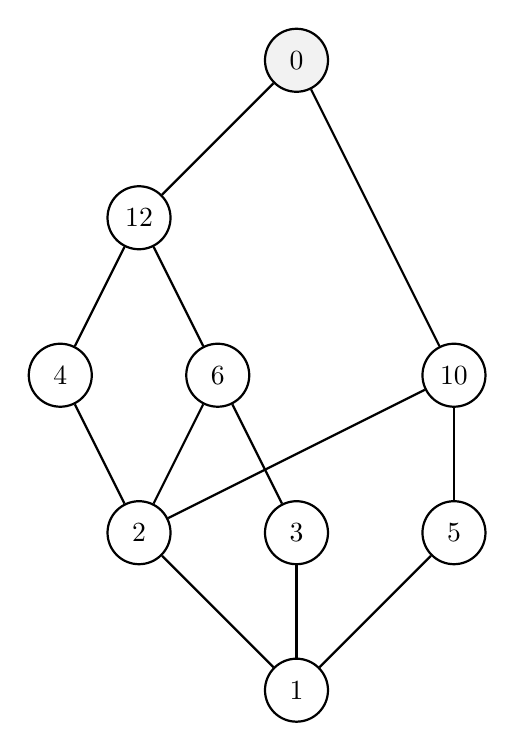
\begin{tikzpicture}[
    number/.style={
        circle, 
        draw=black, 
        thick, 
        minimum size=8mm, 
        inner sep=0pt,
    },
    edge/.style={
        thick,
        draw=black
    }
]

    \node[number] (1) at (0,0) {1};

    \node[number] (2) at (-2, 2) {2};
    \node[number] (3) at (0, 2) {3};
    \node[number] (5) at (2, 2) {5};

    \node[number] (4) at (-3, 4) {4};
    \node[number] (6) at (-1, 4) {6};
    \node[number] (10) at (2, 4) {10};

    \node[number] (12) at (-2, 6) {12};

    \node[number, fill=gray!10] (0) at (0, 8) {0};

    \draw[edge] (1) -- (2);
    \draw[edge] (1) -- (3);
    \draw[edge] (1) -- (5);

    \draw[edge] (2) -- (4); 
    \draw[edge] (2) -- (6); 
    \draw[edge] (3) -- (6); 
    \draw[edge] (2) -- (10);
    \draw[edge] (5) -- (10);

    \draw[edge] (4) -- (12);
    \draw[edge] (6) -- (12);

    \draw[edge] (12) -- (0);
    \draw[edge] (10) -- (0);
\end{tikzpicture}
\caption{Příklad Hasseova diagramu pro přirozená čísla uspořádaná dělitelností.}
\end{figure}
\vspace{-1.5em}
Nula je \enquote{největším} prvkem, protože $0 = k \cdot 0$, tj. platí $a | 0$ pro každé $a$. 

\subsection{Prvočísla}\label{prvocisla}
Přirozené číslo $p \geq 2$ je \ii{prvočíslo}, pokud je dělitelné pouze čísly $1$ a $p$, aneb pokud se nedá napsat jako součin dvou čísel menších než $p$.

Test prvočíselnosti \enquote{hrubou silou}: Číslo $n$ je prvočíslo, pokud není dělitelné beze zbytku žádným prvočíslem $p \leq \sqrt{n}$.

Problém testování prvočíselnosti (resp. rozložení čísla $n$ na součin dvou menších čísel) \enquote{hrubou silou} má exponenciální čásovou složitost v závislosti na počtu cifer čísla $n$. Musíme vykonat
\begin{equation}
	\sqrt{n} = \sqrt{2^{\log_2(n)}} = 2^{\frac{1}{2}\log_2(n)}
\end{equation}
dělení.

Pokud prvočíslo dělí součin dvou čísel, pak dělí alespoň jedno z nich.

\subsection{Věta o nekonečném počtu prvočísel}
\ii{Euklid.} Neexistuje největší prvočíslo, aneb prvočísel je nekonečně mnoho.

\dukaz Ať $P$ je násobek všech prvočísel v seznamu $L = \bc{p_1, p_2, \dots, p_n}$: $P = p_1 p_2 \dots p_n$. Mějme $q = P + 1$, pak
\vspace{-1em}
\begin{itemize}
	\item pokud $q$ je prvočíslo, pak alespoň jedno prvočíslo chybí v seznamu $L$, protože $q \not\in L$;
	\item pokud $q$ není prvočíslo, pak nějaké prvočíslo $p$ dělí $q$. Pokud $p \in L$, tak by $p$ dělilo $P$. Pokud $p$ dělí $P$ a $q$, pak $p$ musí dělit také rozdíl techto dvou čísel, který je $(P + 1) - P$, tedy 1. Jelikož žádné prvočíslo nedělí 1, tak $p \not\in L$. To znamená, že existuje alespoň jedno další prvočíslo, které v $L$ není.
\end{itemize}
\vspace{-1em}
\hspace{\fill}\qed

\subsection{Základní věta aritmetiky}
Každé přirozené číslo $n \geq 2$ lze jednoznačně (až na pořadí) napsat jako součin mocnin různých prvočísel.

\subsection{Největší společný dělitel}\label{gcd}
\ii{Největší společný dělitel} dvou čísel $a, b \in \Z$ je takové číslo $d \in \Z$, které splňuje
\vspace{-1em}
\begin{itemize}
	\item $d$ dělí obě čísla $a$ i $b$,
	\item $d$ je dělitelné všemi společnými děliteli obou čísel,
	\item $d \geq 0$.
\end{itemize}
\vspace{-1em}
Značíme $d = \gcd(a,b)$.

Analogicky lze definovat \ii{nejmenší společný násobek}, $\lcm(a,b)$.

\subsection{Eukleidův algoritmus}\label{eukleidAlgo}
Hledáme $\gcd(a,b)$. Předpokládejme, že $a \geq b > 0$.
\begin{enumerate}[1)]
	\item \hyperref[delZbyt]{Podělíme se zbytkem}: $a = q \cdot b + z$ a $0 \leq z < b$.
	\item Pokud je zbytek $z = 0$, tak je $\gcd(a,b) = b$.
	\item Pokud je zbytek $z > 0$, tak dvojice $a,b$ má stejné společné dělitele jako dvojice $b,z$. Tedy i $\gcd(a,b) = \gcd(b,z)$. Budeme dále hledat $\gcd(b,z)$ stejným postupem.
\end{enumerate}
Jedná se o rekurzivní algoritmus, který se opírá o dělení se zbytkem. Jelikož zbytky jsou celočíselné, nezáporné a stále menší, bude po konečném počtu kroků zbytek nulový (úloha se zastaví). Protože počet dělení se zbytkem je lineární v závislosti na počtu cifer menšího čísla, je časová složitost maximálně kubická.

\subsection{Příklad použití Eukleidova algoritmu}
Určete $\gcd(156, 114)$.
\begin{align}
	\tag{R1} 156 &= 1 \cdot 114 + 42 \\
	\tag{R2} 114 &= 2 \cdot 42 + 30 \\
	\tag{R3} 42 &= 1 \cdot 30 + 12 \\\
	\tag{R4} 30 &= 2 \cdot 12 + 6 \\
	\tag{R5} 12 &= 2 \cdot \boxed{6}  + 0
\end{align}
$\gcd(156, 114) = 6$.

\subsection{Příklad použití Eukleidova algoritmu}
Najděte $\gcd(204, 150)$.
\begin{center}
	\begin{tabular}{r|l}
		$q$ & $a -qb$\\
		1 & $204 = a$ \\
		2 & $150 = \phantom{a +} b$ \\
		1 & $\phantom{1}54 = a - b \rightarrow (a-0a) + (0b -b)$\\
		3 & $\phantom{1}42 = -2a + 3b$ \\
		2 & $\phantom{11}6 = -11a + 15b$ \\
		& \phantom{11}0 
	\end{tabular}
\end{center}

\subsection{Bezoutova věta}\label{bezout}
Největší společný dělitel čísel  $a, b \in \Z$ je jejich celočíselnou kombinací, aneb
\begin{equation}
	\gcd(a,b) = k \cdot a + l \cdot b \quad \text{pro nějaká} \quad k, l \in \Z.
\end{equation}

\subsection{Rozšířený Eukleidův algoritmus}\label{rozEukleidAlgo}
K nalezení celočíselných koeficientů $k, l \in \Z$ z \hyperref[bezout]{Bezoutovy} věty lze použít \ii{rozšířený Eukleidův algoritmus}:
\begin{itemize}
	\item V každém kroku \hyperref[eukleidAlgo]{Eukleidova algoritmu} přepočítáme aktuální zbytek na kombinaci čísel $a,b$.
	\item $\gcd(a,b)$ je posledním nenulovým zbytkem, tudíž jednou nakombinujeme z čísel $a,b$ i jejich \hyperref[gcd]{největšího společného dělitele}.
\end{itemize}

\subsection{Příklad použití Eukleidův algoritmus}
Máme $\gcd(156, 114)$. Označme $a = 156$, $b = 114$.
\begin{align}
	\tag{R1} 42 &= 1a - 1b \\
	\tag{R2} 30 &= 114 - 2 \cdot 42 = b - 2(a-b) = -2a + 3b \\
	\tag{R3} 12 &= 42 - 30 = a - b + 2a - 3b = 3a - 4b \\
	\tag{R4} 6 &= 30 -2 \cdot 12 = -2a + 3b -2(3a - 4b) = -8a + 11b
\end{align}
% TODO: zápis tabulkou

\subsection{Diofantické rovnice}\label{diofantRce}
Rovnice $ax + by = c$, kde $a,b,c \in \Z$, má řešení v $\Z$ právě tehdy, když $\gcd(a,b) | c$.

Pokud nějaké celočíselné řešení diofantické rovnice existuje, pak je jich nekonečné mnoho a jsou tvaru
\begin{equation}
	(x, y) = (x_p, y_p) + k(x_0, y_0) \quad \text{pro} \quad k \in \Z,
\end{equation}
kde $(x_p, y_p)$ je partikulární řešení (najdeme jej pomocí \hyperref[rozEukleidAlgo]{rozšířeného Eukleidova algoritmu}) a $(x_0, y_0)$ je nesoudělné řešení homogenní rovnice, tedy $(x_0, y_0) = (\frac{b}{d}, - \frac{a}{d})$, kde $d = \gcd(a,b)$.
% TODO: příklad

\subsection{Příklad řešení diofantické rovnice}
Řešte diofantickou rovnici
\begin{equation}
	204x + 150y = 36.
\end{equation}
\begin{align}
	x_p &= \gcd(204, 150)x + x_h = -66 + 25k, \\
	y_p &= \gcd(204, 150)y + y_h = 90 - 34k, k \in \Z
\end{align}

\subsection{Příklad řešení diofantickou rovnicí}
Najděte $51^{-1}$ v $\Z_{73}$.
Tedy
\begin{align}
	51x &= 1 \text{ v } \Z_{73} \\
	51x + 73y &= 1 \dots \text{ 51 a 73 jsou nesoudělná, rovnice má tedy řešení.}
\end{align}
\begin{center}
	\begin{tabular}{r|l}
		$q$ & $a -qb$\\
		1 & $73 = a$ \\
		2 & $51 = \phantom{a +} b$ \\
		1 & $22 = a - b$ \\
		3 & $\phantom{1}7 = -2a + 3b$ \\
		2 & $\phantom{1}1 = 7a - 10b$ \\
		& \phantom{1}0 
	\end{tabular}
\end{center}
Takže
\begin{equation}
	51(-10) + 73 \cdot 7 = 1 \\
	51^{-1} = -10 = 63
\end{equation}

\subsection{Příklad řešení diofantic}

\subsection{Kongruence modulo \texorpdfstring{$n$}{n}}\label{kongruenceMod}
Nechť $n \in \N$. Čísla $a,b \in \Z$ jsou \ii{konguentní modulo $n$}, pokud $n | (b-a)$. Značíme $a \equiv b \pmod{n}$.

Tato tvrzení jsou ekvivalentní:
\vspace{-1em}
\begin{itemize}
	\item $a \equiv b \pmod{n}$ právě tehdy, když čísla $a,b$ mají stejný zbytek po dělení číslem $n$,
	\item $a \equiv b \pmod{n}$ právě, když $b = a + kn$ pro $k \in \Z$.
\end{itemize}

\subsection{Relace kongruence modulo \texorpdfstring{$n$}{n}}
Relace \hyperref[kongruenceMod]{kongruence modulo $n$} je relace ekvivalence na množině celých čísel (tj. reflexivní, symetrická a tranzitivní relace).

Důsledkem je, že relace kongruence modulo $n$ rozloží množinu celých čísel na třídy navzájem ekvivalentních prvků, tzv. \ii{zbytkové třídy modulo $n$}, množinu všech zbytkových tříd modulo $n$ značíme
\begin{equation}
	\Z_n = \bc{[0]_n, [1]_n, \dots, [n-1]_n}, \quad \text{kde } [a]_n = \bc{a+kn \middle| k \in \Z}.
\end{equation}

\subsection{Sčítání a násobení s relací kongruence modulo \texorpdfstring{$n$}{n}}
Relace kongruence modulo $n$ je zachována při sčítání a násobení.
Když
\begin{equation}
	a\equiv b \pmod{n} \quad \text{i} \quad c \equiv d \pmod{n}, 
\end{equation}
pak také
\begin{equation}
	a + c \equiv b + d \pmod{n} \quad \text{i} \quad ac \equiv bd \pmod{n}.	
\end{equation}

Důsledek je, že na množině $\Z_n$ můžeme korektně definovat operace sčítání a násobení přes representanty:
\begin{equation}
	[a]_n \oplus [b]_n = [a+b]_n, \quad [a]_n \odot [b]_n = [a \cdot b]_n.
\end{equation}
Díky definici přes repsentanty zdědí operace $\oplus$ a $\odot$ vlastnosti, které měly operace sčítání a násobení na $\Z$.

\subsection{Faktorový okruh zbytkových tříd modulo \texorpdfstring{$n$}{n}}
Trojice $(\Z, \oplus, \odot)$ tvoří komutativní \hyperref[okruh]{okruh} s jednotkou, který se nazývá \ii{faktorový okruh zbytkových tříd modulo $n$}.

V dalším textu zjednodušíme značení:
\[
	(\Z_n = \bc{0, 1, \dots, n-1}, +, \cdot)	
\]

\subsection{Lineární rovnice v \texorpdfstring{$Z_n$}{Zn}}
Lineární rovnice $ax = b$ v $\Z_n$ lze převést na \hyperref[diofantRce]{diofantickou rovnici} následujícími úpravami:
\begin{align}
	ax &= b \text{ v } \Z_n \\
	ax &= b \pmod{n} \text{ v } \Z \\
	ax + ny &=b \text{ v } \Z
\end{align}
Lineární rovnice $ax = b$ má řešení v $\Z_n$ právě, když $\gcd(a,n) | b$. Je-li $x_p$ jedno řešení, pak každé řešení má tvar
\begin{equation}
	x = x_p + k x_0, \, \text{kde } x_0 = \frac{n}{\gcd(a,n)}, \, 0 \leq k < n \gcd(a,n).
\end{equation}
V okruhu $\Z_n$ tak vznikne celkem $\gcd(a,n)$ různých řešení.

\subsection{Těleso \texorpdfstring{$\Z_n$}{Zn}}
Speciálně rovnice $ax = 1$ bude mít řešení v $\Z_n$ právě, když $\gcd(a,b)=1$ (řešením bude inverzní prvek $a^{-1}$ v $\Z_n$).

Důsledkem je, že prvek $a \in \Z_n$ je invertibilní v $\Z_n$ právě, když je $a$ nesoudělné s $n$.

\hyperref[okruh]{Okruh} $(\Z_n, +, \cdot)$ je těleso právě, když $n=p$ je \hyperref[prvocisla]{prvočíslo}.

\section*{Umocňování v $\Z_n$}
Při sčítání a násobení můžeme čísla nahradit jejich zbytky modulo $n$.

Můžeme nějak zmenšit exponent při umocňování modulo $n$?

Čísel v $\Z_n$ je konečně mnoho, výsledky mocnin se musí opakovat:
\begin{equation}
	\text{Existují} \quad k > l \in \N \quad \text{tak, že} \quad a^k = a^l.
\end{equation}
Pokud je $a$ invertibilní v $\Z_n$, získáme odtud $a^{k-l} = 1$. Mocniny čísla $a$ se cyklí s periodou $k-l$.

Jaká je společná perioda pro všechna invertibilní $a \in \Z_n$?

\subsection{Malá Fermatova věta}\label{malaFermat}
Nechť $p$ je \hyperref[prvocisla]{prvočíslo}. Pro každé $a \not= 0$ je $a^{p-1} = 1$ v $\Z_p$.

\subsection{Euler-Fermatova věta}\label{eulerFermat}
Pro každé $a \in \Z_n$, $a$ nesoudělné s $n$, je $a^{\varphi(n)} = 1$ v $\Z_n$.

Aneb je-li základ nesoudělný s $n$, můžeme exponent zmenšit modulo $\varphi(n)$.

\subsection{Eulerova funkce}\label{eulerFun}
\begin{equation}
	\varphi : \N \rightarrow \N: \varphi(n) = \text{ počet čísel mezi 0 až } (n-1) \text{ nesoudělných s }n
\end{equation}
Pro výpočet Eulerovy funkce platí následující vzorce:
\vspace{-1em}
\begin{itemize}
	\item $\varphi(p) = p-1$ pro $p$ \hyperref[prvocisla]{prvočíslo}
	\item $\varphi(p^k) = p^k - p^{k-1} = p^{k-1}(p-1)$ pro $p$ prvočíslo a $k \in \N$
	\item $\varphi(n \cdot m) = \varphi(n) \cdot \varphi(m)$ pro $n,m \in \N$ navzájem nesoudělná
\end{itemize}
\vspace{-1em}
Známe-li prvočíselný rozklad čísla $n$, umíme spočítat $\varphi(n)$, jinak ne.

\subsection{Eulerova věta}\label{euler}
Nechť $(G, \circ)$ je konečná \hyperref[grupa]{grupa} o $n$ prvcích s neutrálním prvkem 1. Pro každé $a \in G$ platí
\begin{equation}
	a^n = \underbrace{a \circ a \circ \dots \circ a}_{n\text{-krát}} = 1 \text{ v } G.
\end{equation}
\hyperref[eulerFermat]{Euler-Fermatova věta} je speciálním případem \hyperref[euler]{Eulerovy věty} aplikované na grupu $(\Z_n^\star, \cdot)$ invertibilních prvků v monoidu $(\Z_n, \cdot)$.
\begin{equation}
	\Z_n^\star = \bc{a \in \Z_n; \, a \text{ je nesoudělné s } n}
\end{equation}
Počet prvků této grupy $|\Z_n^\star| = \varphi(n)$, neutrální prvek je 1.

\subsection{Řád prvku v grupě}\label{radPrvku}
Pro každé $a \in G$ platí $a^n = 1$ v $n$-prvkové \hyperref[grupa]{grupě} $G$. Pro dané $a$ ale nemusí být $n$ tím nejmenším exponentem, na který musíme umocnit, aby vyšlo 1.

Nechť $(G, \circ)$ je konečná grupa s neutrálním prvkem 1, $a \in G$. Nejmenší přirozené číslo $r > 0$ takové, že
\begin{equation}
	a^r = \underbrace{a \circ a \circ \dots \circ a}_{r\text{-krát}} = 1
\end{equation}
se nazývá \ii{řád prvku} $a$ v grupě $G$. Značíme $\ra(a)$.\\
\dukaz
\vspace{-1em}
\begin{itemize}
	\item[$\Leftarrow$:] Nechť $k=m \cdot \ra(a)$. Pak
	\begin{equation}
		a^k = a^{m \cdot \ra(a)} = \left(a^{\ra(a)}\right)^m = 1^m = 1.
	\end{equation}
	\item[$\Rightarrow$:] Nechť $a^k = 1$. Věta \hyperref[delZbyt]{o dělení se zbytkem} zaručuje
	\begin{equation}
		k = q \cdot \ra(a) + z, \, 0 \leq \ < \ra(a).
	\end{equation}
	Takže
	\begin{equation}
		1= a^k = a^{q \cdot \ra(a) + z} = \left(a^{\ra(a)}\right)^q a^z = a^z.
	\end{equation}
\end{itemize}
\hspace{\fill}\qed

Například pro $\Z_9^\star = \bc{1,2,4,5,7,8}$, $|\Z_9^\star| = \varphi(9) = 6$ jsou
\vspace{-1em}
\begin{itemize}
	\item $\ra(8) = 2$;
	\item $\ra(4) = 3$;
	\item $\ra(2) = 6$.
\end{itemize}
Definice pojmu řád prvku $a$ v konečné grupě $G$ je smysluplná, podle \hyperref[euler]{Eulerovy věty} takové číslo existuje a je $\ra(a) \leq G$.

V monoidu je situace jiná; pokud prvek $a$ není invertibilní, pak $a^k \not= 1$ pro každé $k \geq 1$ (jinak by pro dané $k$ byl prvek $a^{k-1}$ inverzním prvkem k prvku $a$).

Známe-li $\ra(a)$ v grupě $G$, usnadní nám to umocňování: při výpočtu $a^k$ můžeme v exponentu počítat modulo $\ra(a)$. 

Je-li grupa aditivní $(G, +)$ s neutrálním prvkem 0, pak řád je nejmenší $r>0$ takové, že
\begin{equation}
	r \cdot a = \underbrace{a + a + \dots + a}_{r\text{-krát}} = 0.
\end{equation}

\subsection{Tvrzení o dělitelnosti řádu prvku}\label{tvrDelRad}
Nechť $(G, \circ)$ je konečná \hyperref[grupa]{grupa}, $a \in G$. Pak $a^k = 1$ v grupě $G$ právě, když $\ra(a) |k$. 

Důsledkem tvrzení je, že řád prvku $\ra(a)$ v konečné grupě $G$ je dělitelem počtu prvků grupy.

Jedná se o důsledek \hyperref[euler]{Eulerovy věty} (kterou jsme pro komutativní grupy dokázali přímo), a předchozího tvrzení. V nekomutativním případě se postupuje obráceně: z \hyperref[lagrange]{Lagrangeovy věty} se odvodí tvrzení, že řád prvku dělí počet prvků grupy, odtud potom Eulerova věta.

\subsection{Příklad na řád prvku}
Mějme grupu $\Z_{47}^*$.
\begin{enumerate}[a)]
	\item Kolik má prvků a jaké to jsou?
	\item $\ra(2) = ?$ 
\end{enumerate}
\begin{enumerate}[a)]
	\item V grupě jsou všechna $\Z$, která jsou invertibilní. 47 je prvočíslo, takže
	\begin{equation}
		| \Z_{47}^* | = \varphi(47) = 46 = 2 \cdot 23.
	\end{equation}
	A $|\Z_{47}^* | = \Z_{47} \setminus \bc{0}$.
	\item Z \hyperref[tvrDelRad]{tvrzení o dělitelnosti řádu prvku} víme, že všechny možné řády $\ra(a) | 46$, tedy
	\begin{equation}
		\ra(a) \in \bc{1, 2, 23, 46}.
	\end{equation}
	Ověrme:
	\begin{align}
		2^2 &= 4 \not= 1 \\
		2^{23} &= 1\\
		2^{46} &= 1 \text{ dle \hyperref[malaFermat]{Malé Fermatovy věty}}
	\end{align}
	Takže $\ra(2) = 23$ v $\Z_{47}^*$.
\end{enumerate}

% pro zajímavost:
\subsection{Lagrangeova věta}\label{lagrange}
Počet prvků libovolné podgrupy $P$ (v konečné \hyperref[grupa]{grupě} $G$) je dělitelem počtu prvků grupy $G$.

Důsledkem je, že \hyperref[radPrvku]{řád prvku} $\ra(a)$ v konečné grupě $G$ je dělitelem počtu prvků grupy.

% pro zajímavost:
\subsection{Cyklická podgrupa}
Je-li $\ra(a) = r$, pak množina $P = \bc{a, a^2, a^3, \dots, a^r = 1}$ tvoří $r$-prvkovou podgrupu \hyperref[grupa]{grupy} $G$. Nazýváme ji \ii{cyklická podgrupa} generovaná prvkem $a$, značíme ji $P = \langle a \rangle$.

\subsection{Vztahy řádu prvku grupy, Eulerovy funkce a cyklické podgrupy}
Nechť $G$ je konečná \hyperref[grupa]{grupa}, $a \in G$. Pak platí
\vspace{-1em}
\begin{itemize}
	\item pokud $d | \ra(a)$, pak $\ra(a^d) = \frac{\ra(a)}{d}$;
	\item $r(a^k) = \frac{\ra(a)}{\gcd(k, \ra(a))}$;
	\item $r(a^k) = \ra(a)$ právě, když $\gcd(k, \ra(a)) = 1$;
	\item podgrupa $P = \langle a \rangle$ má celkem $\varphi(\ra(a))$ prvků řádu $\ra(a)$.
\end{itemize}
Ukažme odvození pro $\Z_9^* = \langle 2 \rangle$.
\begin{itemize}
	\item $4^s = (2^2)^s = \dots = 1$ (poprvé) $\rightarrow s=3$, protože $2^6 = 1$.
	\item $7^s = (2^4)^s = 2^{6k} = 1$ (poprvé) $\rightarrow s=3$, protože $s = 3 = \frac{\lcm(4,6)}{4} = \frac{\frac{4 \cdot 6}{\gcd(4,6)}}{4}= \frac{6}{\gcd(4,6)}$.\\
	Víme, že $6 | (4s)$. Takže $4s = 6k = \lcm(4,6) = \frac{4 \cdot 6}{\gcd(4,6)} = 4 \cdot \underbrace{\frac{6}{\gcd(4,6)}}_{s}$.
\end{itemize}
% TODO: příklad

\subsection{Cyklická grupa}\label{cyklGrupa}\label{generator}
\hyperref[grupa]{Grupa} $(G, \circ)$ se nazývá \ii{cyklická grupa}, pokud pro nějaký prvek $a \in G$ je $G = \langle a \rangle$. Prvek $a$ je \ii{generátor} grupy $G$.

Konečná grupa $G$ o $n$ prvcích je cyklická právě, když obsahuje prvek $a$ řádu $\ra(a) = n$.

Cyklická grupa o $n$ prvcích má celkem $\varphi(n)$ generátorů. Pravděpodobnost, že při náhodné volbě prvku $a \in G$ najdeme generátor, je $\frac{\varphi(n)}{n}$.
% TODO: příklad s podgrupami

\subsection{Hledání generátoru}
Prvek $a$ je \hyperref[generator]{generátor} konečné \hyperref[grupa]{grupy} $G$ o $n$ prvcích právě, když je splněna některá z podmínek:
\vspace{-1em}
\begin{itemize}
	\item $a^r \not=1$ pro každé $r < n$, kde $r | n$;
	\item $a^r \not=1$ pro každé $r = \frac{n}{p}$, kde $p$ je \hyperref[prvocisla]{prvočíslo} a $p | n$.
\end{itemize}
Například mějme $\Z_{47}^*$. Ověřte, jestli se jedná o cyklickou grupu.

Víme $|\Z_{47}^*| = 46 = 2 \cdot 23$, a také víme, že řády dělí velikost grupy, tedy $r|46$. To nám dává $r \in \bc{1, 2, 23, 46}$. Z předchozích příkladů víme, že $2^{23} = 1 \rightarrow \ra(2) = 23 \rightarrow$ 2 není \hyperref[generator]{generátor}.
Zkusme další číslo, třeba $3$. Hledáme situaci, kdy $a \in \Z_{47}^*:\: a^r \not= 1$. Díky \hyperref[eulerFermat]{Euler-Fermatově větě} ale víme, že $a^{p-1} = 1$ v $\Z_p$, takže $2^{46} = 1$.

Zkusme druhou podmínku s $\Z_{19}^*$.
Víme, že $|\Z_{19}^*| = \varphi(19) = 18$, $\Z_{19}^* = \Z_{19} \setminus \bc{0}$. Víme, že $\ra(a) \in \bc{1, 2, 3, 6, 9, 18}$.

Zkusme $a=2$. Napišme pomocný vztah $0 = 19 = 38 = 57$.
\begin{align}
	2^2 &= 4 \not=1 \\
	2^3 &= 8\not= 1\\
	2^6 &= 8^2 - 64 = 7 \not= 1\\
	2^9 &= 7 \cdot 8 = 56 = 18 = (-1) \not= 1\\
	2^{18} &= (-1)^2 = 1 \text{ (poprvé)}
\end{align}
Takže $\ra(2) = 18 \implies \Z_{19}^* = \langle 2 \rangle$.

\subsection{Tvrzení o komutativní grupě a jejím řádu}
Nechť $G$ je konečná komutativní \hyperref[grupa]{grupa}, $a, b \in G$. (Resp. nechť $ab = ba$.)

Pokud jsou $\ra(a)$ a $\ra(b)$ nesoudělné, pak $\ra(ab) = \ra(a) \ra(b)$.

\subsection{Příklad hledání generátoru}
Je dána \hyperref[grupa]{grupa} $\Z_{19}^* = \Z_{19} \setminus \bc{0}$. Pak $|\Z_{19}^*| = \varphi(19) = 18 = 2 \cdot 3^2$. Možné řády jsou $\ra(a) \in \bc{1, 2, 3, 6, 9, 18}$.

Určete $\ra(8)$ a použijte ho při výpočtu $8^{195}$ v $Z_{19}$.\\
$8^6 = 1$ poprvé, tedy $\ra(8) = 6$. A $8^{195} = 8^3 = 18$ v $\Z_{19}$.

Najděte \hyperref[generator]{generátor} v $\Z_{19}^*$.\\
Zkusme $a=2$. $2^6 = 7 \not=1$ (odtud také $2^2 \not=1$, $2^3 \not=1$), $2^9 = -1 \not=1$, tudíž $\ra(2)=18$ a $2$ je generátor v $\Z_{19}^*$.

Pravděpodobnost náhodné volby generátoru je $P = \frac{\varphi(18)}{18} = \frac{1}{3}$.

\subsection{Příklady cyklických grup}
\vspace{-1em}
\begin{itemize}
	\item \hyperref[grupa]{Grupa} $(\Z_n, +)$ je \hyperref[cyklGrupa]{cyklická} s \hyperref[generator]{generátorem} 1 pro každé $n \geq 1$.
	\item Grupa $(\Z_p^*, \cdot)$ je cyklická pro každé $p$ \hyperref[prvocisla]{prvočíslo}. 
	\item Grupa $(\Z_9^*, \cdot)$ je cyklická s generátorem 2. 
	\item Grupa $(\Z_8^* = \bc{\pm1, \pm3}, \cdot)$ není cyklická grupa, neboť $a^2 = 1$ pro každé $a \in \Z_8^*$. 
\end{itemize}

\subsection{Vnitřní struktura cyklických grup}
Nechť $G = \langle a \rangle$ je \hyperref[cyklGrupa]{cyklická grupa} o $n$ prvcích s neutrálním prvkem 1. Nechť $r | n$, tehdy a jen tehdy platí:
\vspace{-1em}
\begin{enumerate}[a)]
	\item V grupě $G$ lze nalézt prvek řádu $r$, například prvek $b = a^k$, kde $k = \frac{n}{r} \in \N$.
	\item V grupě $G$ je právě jedna podgrupa o $r$ prvcích; a to podgrupa $P_r = \langle b\rangle$, kde $\ra(b) = r$.
	\item Rovnice $x^r = 1$ má v grupě $G$ právě $r$ řešení, a jsou to všechny prvky z $r$-prvkové podgrupy $P_r$. Jsou tedy tvaru $x = b^i$, kde $\ra(b) = r$ a $0 \leq i \leq r-1$.
	\item Pro libovolné $k \in \N$ má rovnice $x^k = 1$ v grupě $G$ právě $d = \gcd(k, n)$ řešení a redukuje se na rovnici $x^d = 1$.
\end{enumerate}

\subsection{Příklad řešení rovnice v grupě}
Řešte rovnici $x^{21} = 1$ v grupě $\Z_{19}^*$.
\begin{enumerate}[a)]
	\item Již víme, že $|\Z_{19}^*| = \varphi(19) =18$ a 2 je generátor v $\Z_{19}^*$.
	\item Prvek $a$ řeší rovnici $x^{21} = 1$ právě, když $\ra(a)|21$. Navíc $a \in \Z_{19}^*$, tudíž $\ra(a) | 18$. Odtud $\ra(a) | \gcd(21, 18) = 3$ a rovnice se redukuje na rovnici $x^3 =1$.
	\item Najdeme prvek $b$ řádu 3: $b=2^{\frac{18}{3}} = 2^6 = 7$. Rovnice má tři řešení, $x_1 = 7$, $x_2 = 7^2 = 49 = 11$, $x_3 = 7^3 = 1$.
	\item Tyto tři prvky jsou kořeny polynomu $x^3 - 1$ v $\Z_{19}$. Protože $(\Z_{19}, +, \cdot)$ je \hyperref[teleso]{těleso}, tak polynom nemůže mít více kořenů, než je jeho stupeň.
\end{enumerate}
